\begin{appendices}

\counterwithin{figure}{section}
\counterwithin{table}{section}

% \section{Glossary}

% \begin{itemize}
%     \item \textbf{Power} The rate at which work is done, energy over time. Measured in Watts (\SI{}{\watt}, \SI{}{\kilo\watt}, \SI{}{\mega\watt}, \SI{}{\giga\watt}).
%     \item \textbf{Energy} An amount of work, measured in Joules or Watt-hours (\SI{}{\watt\hour}, \SI{}{\kilo\watt\hour}, \SI{}{\mega\watt\hour}).
%     \item \textbf{Electricity} Energy transmitted from power plants to consumers over the grid. A subset within the general more category ``energy'', which includes things like heating and fuel for transportation.
%     \item \textbf{Emissions} Greenhouse gas byproducts, mainly {\COtwo}.
%     \item \textbf{Emissions factor} How many greenhouse gases are emitted when producing a given amount of energy (or electricity).
% \end{itemize}

\section{GPU Count}
\label{appendix:gpu-count}

\begin{figure*}[htp]
    \centering
    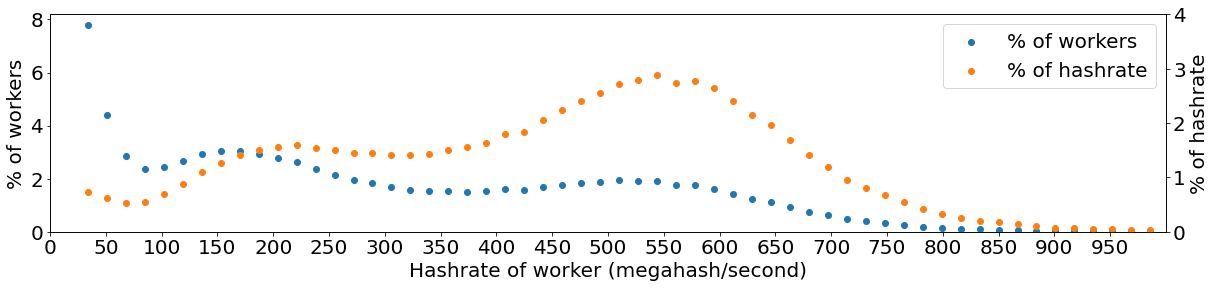
\includegraphics[width=\linewidth]{nanopool-hashrate-analysis}
    \caption{Analysis of the hashrate distribution of around 70,000 active Nanopool workers per day over 4 days.}
    \label{fig:nanopool-hashrate-analysis}
\end{figure*}

Analyzing the hashrate distribution of Nanopool workers reveals a pattern shown in \textbf{figure \ref{fig:nanopool-hashrate-analysis}}: around \var{workers_under_50} of workers have a hashrate under \hr{50}, and \var{workers_under_100} of workers have a hashrate under \hr{100}. This range represents the single-GPU configuration (the fastest GPUs are around \hr{100}). The next peak is around \hr{150}, likely representing the dual-GPU configuration, and the last peak is much wider around \hr{550} likely representing $6\times$ GPU configurations. While there are many few-GPU workers, workers with a hashrate under \hr{100} only represent \var{hashrate_under_100} of the total hashrate, while workers with a hashrate between \hr{100} and \hr{350} represent \var{hashrate_between_100_350} of the total hashrate, and workers over \hr{350} represent the remaining \var{hashrate_above_350}.

\section{Emissions Factors}
\label{appendix:emissions-factors}

\begin{table*}[htp]
\centering
\begin{tabular}{@{}lrrrrrrr@{}}
\toprule
Region               & 2015 & 2016 & 2017 & 2018 & 2019 & 2020 & 2021 \\ \midrule
Asia                 & 666  & 651  & 638  & 623  & 609  & 595  & 581  \\
Singapore            & 422  & 423  & 421  & 420  & 408  & 409  & 406  \\
Taiwan               & 525  & 530  & 554  & 533  & 509  & 521  & 518  \\
South Korea          & 527  & 521  & 537  & 533  & 506  & 472  & 483  \\
China                & 650  & 627  & 623  & 613  & 598  & 580  & 570  \\
China (Northwest)    & 668  & 661  & 653  & 646  & 639  & 632  & 625  \\
China (South)        & 46   & 45   & 44   & 42   & 41   & 40   & 39   \\
Europe               & 313  & 302  & 301  & 288  & 253  & 231  & 224  \\
Sweden               & 10   & 10   & 10   & 11   & 10   & 9    & 9    \\
Netherlands          & 506  & 487  & 460  & 440  & 392  & 328  & 316  \\
Germany              & 448  & 445  & 413  & 404  & 344  & 311  & 294  \\
Russia               & 326  & 327  & 325  & 325  & 323  & 301  & 307  \\
Ukraine              & 372  & 400  & 337  & 342  & 342  & 333  & 317  \\
United States        & 467  & 419  & 431  & 408  & 401  & 386  & 370  \\
United States (East) & 410  & 389  & 368  & 350  & 325  & 305  & 284  \\
United States (West) & 534  & 510  & 495  & 492  & 446  & 437  & 417  \\ \bottomrule
\end{tabular}
\caption{Regional emissions factor estimates, in \ef{}}
\label{tab:emissions-factors}
\end{table*}

An emissions factor is the ratio between \COtwo{} emissions and energy production. It is most often expressed as \ef{} or \SI{}{\kilo\gram\COtwo\per{\mega\watt\hour}} in a 0-1000 range, or as \SI{}{\ton\COtwo\per{\mega\watt\hour}} in a 0-1 range. The IPCC estimates\cite{ipcc_annex_2014} that the average emissions factor is \ef{961} for electricity generated by coal plants, and \ef{483} for gas plants, while renewables like wind and hydro emit less than \ef{10}\cite{moomaw_annex_2012} over their lifetime (due to construction and operation). An emissions factor can be used to estimate how much \COtwo{} was emitted while generating a given amount of power.

The IEA tracks and sells global emissions factors\cite{iea_emissions_2021}, but does not allow them to be published, making any derived work impossible to openly audit. To make this work auditable, we have estimated historical emissions factors for multiple regions relevant to Ethereum mining. We have also had a third party compare our emissions factors to the IEA emissions factors.

When an emissions factor is not directly available from a governmental authority, it may be estimated by:

\begin{itemize}
    \item Dividing total electricity emissions statistics by total electricity generation statistics.
    \item Taking a weighted average of the emissions factors for different energy sources in a grid (the energy mix), in proportion to the electricity generated by each source.
    \item Assuming that changes in emissions factors are relatively smooth, we may fit a line and interpolate between or extrapolate beyond known emissions factors.
\end{itemize}

Collecting and estimating emissions factors requires navigating ancient and byzantine energy agency websites, and searching for obscure presentations that include a few well-researched data points. The latest data is often a few years old. Sometimes numbers that initially look like electricity generation emissions factors turn out to actually include heating in addition to electricity, or they are projected future emissions factors accounting for power plants under construction.

We use government-reported emissions factors where possible, augmented with historical energy mix statistics, and some extrapolation and interpolation for missing data. Of all our emissions factors, 38\% are government-reported, 24\% are based on energy mix statistics, 23\% are interpolated, and 14\% are provided by non-governmental entities like the IEA.

Calculating regional emissions factors would be a straightforward process if every region had an electric grid that was completely isolated from its neighbors. In reality, grids are often connected between countries and states using a complex web of high voltage lines. These connections are managed by transmission system operators (TSOs). When electricity is purchased, it is usually bought within the scope of a TSO boundary. When the EPA gives an emissions factor of \ef{875} for the state of West Virginia in 2019, this is based on all the power plants operating in the state rather than within the TSO boundary. West Virginia is located in a RFCW TSO region, which has an emissions factor of \ef{484}.

\begin{itemize}

    \item \textbf{Asia} The IEA\cite[65]{iea_co2_2019} provides estimates for ``\ef{} of electricity'' within ``Non-OECD Asia (excluding China)'' as \ef{666} in 2015 and \ef{638} in 2017. Other years are interpolated and extrapolated. These emissions factors are designed to capture the presence of crypto mining in Southeast Asian countries like Cambodia and Vietnam\cite{redman_chinese_2018}.
    
    \item \textbf{China} We use the IEA\cite{iea_development_2020} estimates for China 2015-2020, 2021 is extrapolated. We also cross-check these numbers against the EIA\cite{us_eia_international_2021} which estimates Chinese electric generation from fossil fuels during 2015-2019 slowly dropping from 72\% to 67\%. Under the assumption that the energy mix within fossil fuels has stayed consistent, the EIA percentages match the IEA estimates within $\pm1\%$.
    
    \item \textbf{China (Northwest)} Tao et al.\cite{tao_measuring_2016} provides ``revised electric power emission factors'' for each grid region in China, approximating the complexities of emissions responsibilities implied by interprovincial power dispatching. They estimate emissions factors for all six regions from 2000-2015. We fit a line to these factors and predict 2015-2021. These predictions might be cross-referenced against Chinese Ministry of Ecology and Environment (MEE) numbers for regional grid baseline emissions factors\cite{yu_baseline_2020}. But because Tao is accounting for energy import and export, and the MEE does not, the numbers do not match. As an example, the MEE estimates Northwest China at \ef{892} during 2015-2017, while a line fit from Tao averages \ef{661} during that same period. In general, our emissions factors are low compared to the MEE estimates. Our factors are comparable to Li et al.\cite{li_life_2018} which estimates \ef{650} for 2020 while we estimate \ef{632}.
    
    \item \textbf{China (South)} We use the same methodology as \textbf{China (Northwest)} but scale our predictions based on the energy mix in the wet season. Models from Liu and Davidson\cite{liu_china_2021} indicate that in Yunnan during the wet seasons 2016-2019, coal only contributed roughly 4\% to 6\% of the total electricity generation. Given that Chinese electricity in 2017 was 70\% fossil fuels\cite{us_eia_international_2021} and mostly coal, and that the 2017 emissions factor was \ef{623}\cite[67]{iea_co2_2019} we can estimate Chinese fossil fuels to emit roughly \ef{890}, similar to the \ef{870} given by Ademe\cite{baude_key_2020} or the \ef{913} minimum from the IPCC\cite{ipcc_annex_2014}. Assuming 5\% coal in Yunnan during the wet season gives us an emissions factor of $5\%\times\ef{890}=\ef{44}$. Scaling the line fit from Tao gives us a final result of \ef{46} in 2015 dropping to \ef{39} in 2021. These factors are designed to capture the very low emissions associated with electricity generation in Sichuan and Yunnan from an abundance of hydropower. These wet season numbers are lower than the annual \ef{80} to \ef{200} range given by Li et al. for 2020 in Sichuan, and much lower than the annual \ef{225} to \ef{155} range given by a line fit from Tao et al. over 2015-2021. Both Sichuan and Yunnan are part of larger TSO regions, the Central and Southern power grids, which have much higher emissions. We use local emissions instead of TSO-wide emissions because the low price of electricity in this region indicates that it is due to an inability to efficiently export the power.
    
    \item \textbf{Europe} The EEA\cite{eea_greenhouse_2021} estimates ``greenhouse gas emission intensity of electricity generation'' for the European Union as declining from \efe{313} in 2015 to \efe{231} in 2020. While \COtwoe{} emissions cover more greenhouse gases than \COtwo{}, these numbers closely match the IEA\cite{iea_development_2020}. We extrapolate for 2021.
    
    \item \textbf{Germany}, \textbf{Netherlands} and \textbf{Sweden} We use the EEA\cite{eea_greenhouse_2021} estimates for 2015 to 2020, and extrapolate for 2021. The national borders of Sweden matches their TSO borders (Svenska kraftnät), while the Netherlands TSO TenneT extends into Germany which is served by three additional TSOs\cite{wikipedia_contributors_european_2021}.
    
    \item \textbf{Russia} BP\cite{bp_statistical_2021} provides electricity generation statistics for Russia including from oil, gas, coal, and total. According to the state-owned Russian energy corporation Gazprom\cite{gazprom_pjsc_2019}, emissions factors are \ef{400} for gas, \ef{600} for oil and \ef{845} to \ef{1020} for coal. We weight the yearly electricity generation statistics by these numbers, using the lower end \ef{845} for coal, and divide by the total generated electricity. For example, in 2018:

    \begin{align*}
    e_{gas} & = \ef{400}\times\SI{523}{\TWh} \\
    e_{oil} & = \ef{600}\times\SI{7.9}{\TWh} \\
    e_{coal} & = \ef{845}\times\SI{176}{\TWh} \\
    f_{mix} & = \frac{e_{gas}+e_{oil}+e_{coal}}{\SI{1109}{\TWh}} \\
     & = \ef{327}
    \end{align*}

    Similar to \ef{325} estimated for 2018 by Enerdata\cite{enerdata_market_2021}, reported by Carbon Footprint\cite{carbon_footprint_carbonfootprintcom_2020} from the Climate Transparency Report\cite{climate_transparency_brown_2018}. We apply this small scaling factor to the weighted estimates, and extrapolate to 2021. These numbers are comparable and lower than the Gazprom estimate \ef{358} for the earlier 2010-2016 period\cite[50]{gazprom_pjsc_2019}. This also matches the trend reported by the European Bank for Reconstruction and Development\cite{schreider_development_2011}, which predicted that Russian emissions would remain nearly unchanged between 2009-2020. Finally, percentages derived from BP's data give identical results to the EIA energy mix percentages: both give 64\% fossil fuels for 2018.
    
    \item \textbf{Singapore} We use the Energy Market Authority of the Singapore Government\cite{energy_market_authority_singapore_2021} data for 2015-2019. 2020 and 2021 are extrapolated.
    
    \item \textbf{South Korea} We use the IEA\cite{iea_development_2020} estimates for South Korea 2015-2020, 2021 is extrapolated.
    
    \item \textbf{Taiwan} We use the Taiwan Bureau of Energy 2020 Energy Statistics Handbook for 2015-2019\cite[17]{taiwan_bureau_of_energy_energy_2020} and extrapolate for 2020 and 2021.
    
    \item \textbf{Ukraine} We use the EIA fossil fuel percentage estimate from 2010-2020. We then use two equally weighted datapoints from The Climate Registry\cite{the_climate_registry_default_2021}: \ef{392} in 2010 and \ef{450} in 2011. These datapoints imply between \ef{860} to \ef{941} for fossil fuel based emissions in Ukraine. This generally matches other statistics\cite{wikipedia_contributors_energy_2021}\cite{the_shift_project_shift_2020} that report Ukraine's fossil fuel energy mix around 80\% coal and increasing since 2010. We extrapolate for 2021.
    
    \item \textbf{United States} We use the EPA eGRID data for 2018 and 2019\cite{us_epa_data_2020}. We divide the total emissions by the total generation across all regions. For example, in 2019 the US emitted \SI{1.83}{\giga\ton\COtwo} (short tons\footnote{The EPA reports \COtwo{} emissions in units of ``short tons'' equivalent to 2000 pounds, or around \SI{907}{\kilo\gram}}) for \SI{4,140}{\TWh}, around \SI{0.442}{\ton\COtwoe\per{\mega\watt\hour}} (short tons), or \ef{401}. We can use the same technique to estimate the emissions for 2016 using the eGRID 2016 Summary Tables\cite{us_epa_download_2020}. For 2020 we use EIA fossil fuel percentages. First we estimate an emissions factor for fossil fuels in 2019 as \ef{646}, given the \ef{401} overall emissions factor and 61\% fossil fuels statistic. We multiply that by the 59\% fossil fuels percentage for 2020 to get \ef{386} for 2020. We repeat this for 2015 using 2016, and for 2017 using 2016 and 2018. Finally, we extrapolate from this data to 2021.
    
    \item \textbf{United States (West)} and \textbf{United States (East)} Recent research\cite{sigalos_bitcoin_2021} indicates that 80\% Bitcoin mining in the USA happens in New York (NYUP), Kentucky (SRTV), Georgia (SRSO), Texas (ERCT) and Nebraska (MROW). We assume that Ethereum follows a similar pattern. We assign Nebraska and Texas as representing the West, and the others for the East. We use EPA eGRID data for 2018 and 2019 and eGRID 2016 Summary Tables for each of the corresponding TSO regions, and take the average across the regions. 2015, 2017, and 2020-2021 are extrapolated.

\end{itemize}

\section{Mining Regions}
\label{appendix:mining-regions}

When the region of a block cannot be estimated from its \texttt{extraData} field, we use the mining pool to estimate where it was mined. Some of the largest mining pools have multiple international servers, and others have fewer servers or have users that are geographically concentrated. We map mining pools to one or more of five regions: \texttt{asia}, \texttt{china}, \texttt{europe}, \texttt{russia}, \texttt{us}. \texttt{asia} refers to mining pools that are used broadly across Asia (including China, Japan, South Korea, and throughout Southeast Asia), while \texttt{china} is meant for pools used primarily by Chinese miners.

\begin{table}[htp]
\centering
\begin{tabular}{@{}llll@{}}
\toprule
Miner & \texttt{europe} & \texttt{us} & \texttt{asia} \\ \midrule
2Miners & 95 & 4 & 1 \\
Bw Pool & 32 & 10 & 58 \\
Coinotron & 92 & 8 &  \\
DwarfPool & 84 & 12 & 4 \\
Ethermine & 72 & 15 & 13 \\
F2Pool & 23 & 10 & 67 \\
firepool & 27 & 13 & 60 \\
Hiveon & 85 & 14 & 1 \\
Huobi Mining Pool & 49 & 25 & 26 \\
Nanopool & 94 & 6 &  \\
PandaPool & 24 & 11 & 65 \\
Spark Pool & 20 & 10 & 70 \\
UUPool & 6 & 4 & 90 \\
xnpool.cn & 32 & 14 & 54 \\
zhizhu.top & 24 & 9 & 67 \\ \bottomrule
\end{tabular}
\caption{An excerpt of mappings from mining pools to regions based on data from Silva et al\cite{silva_impact_2020}.}
\label{tab:mining-pool-regions}
\end{table}

Pool region distribution estimates are based on:

\begin{itemize}
    \item \textbf{Block propagation delay} During a one-month period from 2019-04-01 to 2021-05-02, Silva et al\cite{silva_impact_2020} logged activity on the Ethereum network using four servers. The servers were located in Portugal, Czech Republic, Taiwan, and the USA. When a block is mined by a pool in China, the block will first be reported to servers in Taiwan before it is reported to servers in the USA. For example, 94\% of Nanopool-mined blocks arrived in Portugal or Czech Republic before other regions, so we weight Nanopool as 94\% \texttt{europe}. And 90\% of UUPool-mined blocks arrived in Taiwan before other regions, so we weight UUPool as 90\% \texttt{asia}. We map 15 pools this way.
    \item \textbf{Mining Pool Stats}\cite{miningpoolstats_ethereum_2021} Regions for many current pools are listed on this tracking website. Sometimes the regions are overly general (e.g. ``global'') and can be narrowed down.
    \item \textbf{Language} Website localization options can be a clue to the user base. For example \texttt{xnpool} only offers a Chinese language interface.
    \item \textbf{Server locations} For example SpiderPool only offers servers in Hangzhou, Chengdu, and Hohhot (\texttt{eth.pool.zhizhu.top}, \texttt{eth-cd}, \texttt{eth-nmg}). While F2Pool offers servers in China, North America, and Europe (\texttt{eth.f2pool.com},  \texttt{eth-na}, \texttt{eth-eu}).
\end{itemize}

\section{Region Mapping}
\label{appendix:region-mapping}

\newcommand{\diag}[1]{\multicolumn{1}{l}{\rlap{\rotatebox{60}{#1}~}}} 

\begin{table*}[!htpb]
\centering
\begin{tabular}{@{}lllllllllllllllll@{}}
label & \diag{Asia} & \diag{Singapore} & \diag{Taiwan} & \diag{South Korea} & \diag{China} & \diag{China (Northwest)} & \diag{China (South)} & \diag{Europe} & \diag{Sweden} & \diag{Netherlands} & \diag{Germany} & \diag{Russia} & \diag{Ukraine} & \diag{United States} & \diag{United States (East)} & \diag{United States (West)} \\
\texttt{asia} & \multicolumn{1}{r}{10} & \multicolumn{1}{r}{2} & \multicolumn{1}{r}{1} & \multicolumn{1}{r}{3} & \multicolumn{1}{r}{16} & \multicolumn{1}{r}{32} & \multicolumn{1}{r}{32} &  &  &  &  &  &  &  &  &  \\
\texttt{singapore} &  & \multicolumn{1}{r}{1} &  &  &  &  &  &  &  &  &  &  &  &  &  &  \\
\texttt{taiwan} &  &  & \multicolumn{1}{r}{1} &  &  &  &  &  &  &  &  &  &  &  &  &  \\
\texttt{seoul} &  &  &  & \multicolumn{1}{r}{1} &  &  &  &  &  &  &  &  &  &  &  &  \\
\texttt{china} &  &  &  &  & \multicolumn{1}{r}{1} & \multicolumn{1}{r}{2} & \multicolumn{1}{r}{2} &  &  &  &  &  &  &  &  &  \\ \midrule
\texttt{europe} &  &  &  &  &  &  &  & \multicolumn{1}{r}{2} & \multicolumn{1}{r}{6} & \multicolumn{1}{r}{2} & \multicolumn{1}{r}{1} &  &  &  &  &  \\
\texttt{europe-west} &  &  &  &  &  &  &  & \multicolumn{1}{r}{2} &  & \multicolumn{1}{r}{6} & \multicolumn{1}{r}{1} &  &  &  &  &  \\ 
\texttt{europe-north} &  &  &  &  &  &  &  & \multicolumn{1}{r}{2} & \multicolumn{1}{r}{6} &  & \multicolumn{1}{r}{1} &  &  &  &  &  \\ \midrule
\texttt{russia} &  &  &  &  &  &  &  &  &  &  &  & \multicolumn{1}{r}{3} & \multicolumn{1}{r}{1} &  &  &  \\
\texttt{ukraine} &  &  &  &  &  &  &  &  &  &  &  & \multicolumn{1}{r}{1} & \multicolumn{1}{r}{3} &  &  &  \\ \midrule
\texttt{us} &  &  &  &  &  &  &  &  &  &  &  &  &  & \multicolumn{1}{r}{2} & \multicolumn{1}{r}{5} & \multicolumn{1}{r}{3} \\
\texttt{us-east} &  &  &  &  &  &  &  &  &  &  &  &  &  & \multicolumn{1}{r}{1} & \multicolumn{1}{r}{4} &  \\
\texttt{us-west} &  &  &  &  &  &  &  &  &  &  &  &  &  & \multicolumn{1}{r}{1} &  & \multicolumn{1}{r}{4}
\end{tabular}
\caption{Mapping from \texttt{extraData} regions and mining pool regions to electric grids.}
\label{tab:regions-to-grids}
\end{table*}

In order to convert \texttt{extraData} regions and mining pool regions to emissions factors, we need to make an informed guess. For each \texttt{extraData} region, where are the miners located that are connecting to that server? And for each mining pool region, where are the miners located that are using that mining pool?

\begin{itemize}

    \item \textbf{\texttt{asia}} From looking at the \texttt{extraData} alone, Ethereum mining in Asia is dominated by users connecting to servers in China. Around 82\% of blocks mined by an Asian server were submitted by a Chinese server. Another 10\% of blocks were submitted by a server indicating ``\texttt{asia}'' in the \texttt{extraData}. The remaining 3.5\%, 2.2\% and 1\% of blocks were mined by servers indicating \texttt{seoul}, \texttt{singapore} or \texttt{taiwan} respectively. We assume that users connecting to an \texttt{asia} server or an \texttt{asia}-based mining pool will follow this same distribution. Within China we use a $2:2:1$ ratio based on observations of Bitcoin by CBECI indicating that over the 12 month period from 2020-07-01 to 2021-07-01, mining in the Southern provinces of Sichuan and Yunnan made up 42\% of all Chinese mining activity, while mining in Xinjiang made up 36\% and other regions made up 21\%. This definition of \texttt{asia} is useful before the 2021-05-21 ban in China, but future work should update this definition to account for the new mix.

    \item \textbf{\texttt{singapore}}, \textbf{\texttt{taiwan}} and \textbf{\texttt{seoul}} We map these regions directly to their corresponding national grid.
    
    \item \textbf{\texttt{china}} We use a $2:2:1$ ratio between the Southern and Northwestern provinces and China as a whole, same as used in \texttt{\textbf{asia}}.
    
    \item \textbf{\texttt{europe}} Under the assumption that most European mining happens in places with below-average electricity prices, like Sweden (and Norway, and Iceland), we map \textbf{\texttt{europe}} evenly between these grids in a $6:1$ ratio with Europe as a whole.
    
    \item \textbf{\texttt{europe-west}} We map this primarily to Netherlands, based on statistics from cloud mining platform Mining Rig Rentals\cite{mining_rig_rentals_dagger-hashimoto_2021}. Scraping 2700 mining rigs rental listings, we found that the most common listings in Europe were located in Amsterdam (710) and Germany (563), followed by the UK (34). Because electricity in Germany is priced 50\% higher than the European average\cite{eurostat_fileelectricity_2021}, it is possible that these mining rigs are using a network proxy, and are physically located outside of Germany. CBECI has also written about apparent Bitcoin mining in Germany, ``there is little evidence of large mining operations in Germany [...] that would justify these figures. Their share is likely significantly inflated due to redirected IP addresses via the use of VPN or proxy services.''
    
    \item \textbf{\texttt{europe-north}} We map this primarily to Sweden, which has very low emissions factor and cheap electricity at 60-70\% of the European average price of \eurkwh{0.11}\cite{steitz_cryptocurrency_2018} in 2018: \eurkwh{0.065} in Sweden, \eurkwh{0.071} in Norway, and \eurkwh{0.08} in Iceland.
    
    \item \textbf{\texttt{russia}} and \textbf{\texttt{ukraine}} We assume that a portion of Russian miners connect to Ukranian servers and vice versa.
    
    \item \textbf{\texttt{us}}, \textbf{\texttt{us-east}} and \textbf{\texttt{us-west}} We balance $5:3$ in favor of \texttt{us-east} when allocating across the entire USA based on indicators from \texttt{extraData}. For the West and East we guess that 20\% is from outside the mapped regions.
    
\end{itemize}

\end{appendices}